\documentclass[10pt,a4paper]{article}
\usepackage[utf8]{inputenc}
\usepackage[T1]{fontenc}
\usepackage{amsmath}
\usepackage{amsfonts}
\usepackage{amssymb}
\usepackage{graphicx}
\graphicspath{ {Imagenes/} }
\usepackage{wrapfig}
\usepackage{fancyhdr}
\usepackage{enumitem}
\usepackage{vmargin}

\setpapersize{A4}
\setmargins{2.5cm}       % margen izquierdo
{1.5cm}                        % margen superior
{16.5cm}                      % anchura del texto
{23.42cm}                    % altura del texto
{10pt}                           % altura de los encabezados
{1cm}                           % espacio entre el texto y los encabezados
{0pt}                             % altura del pie de página
{2cm}                           % espacio entre el texto y el pie de página
\begin{document}
	\title{TEMA 3: CIRCUITOS EN CORRIENTE ALTERNA}
	\date{}
	\author{}
	\maketitle
	
	\section{Introducción: CA vs. CC}
	
	\begin{itemize}
		\item CA: facilidad de transformación.
		\item Elevación de tensión en CC $\implies$ conexión de generadores en serie $\implies$ poco práctico.
		\item Elevación de tensión en CA $\implies$ uso de transformadores $\implies$ eficiente.
		\item Energía transportada: $I = vit$. La misma energía puede ser distribuida a largas distancias con bajas intensidades de corriente y, por tanto, con bajas pérdidas ($U_{perdidas} = Ri^2t$).
		\item Una vez en el punto de consumo, el voltaje se puede reducir de nuevo para su uso.
	\end{itemize}
	
	\section{Fasores y números complejos}
	
	Si $v(t) = V_0 e^{j (\omega t + \alpha)} \implies$ si $V = V_0 e^{j \alpha} \implies v(t) = V e ^{j \omega t}$. \newline
	
	Es un número complejo que representa el módulo $V_0$ yy la fase inicial $e ^{j \alpha}$ de una señal sinusoidal $v(t)$.
	
	\section{Impedancia}
	
	Ley de Ohm generalizada:
	$$\boxed{v(t) = Z i(t)}$$
	
	\subsection{Resistencia}
	
	\begin{itemize}
		\item $v(t) = R i(t)$
		\item $Z_R = R$
		\item $i(t) = \dfrac{V_0}{R}e^{j(\omega t + \alpha)}$
	\end{itemize}
	
	\subsection{Condensador}
	
	\begin{itemize}
		\item $i(t) = C \dfrac{dv(t)}{dt}$
		\item $Z_C = \dfrac{1}{j\omega C} = \dfrac{-j}{\omega C} = \dfrac{1}{\omega C} e^{-j\tfrac{\pi}{2}}$
		\item $i(t) = Cj\omega v(t) = C \omega V_0 e^{j(\omega t + \alpha + \tfrac{\pi}{2})}$
	\end{itemize}

	\subsection{Bobina}
	
	\begin{itemize}
		\item $v(t) = L \dfrac{d i(t)}{dt}$
		\item $Z_L = j \omega L = \omega L e ^{j \tfrac{\pi}{2}}$
		\item $i(t) = \dfrac{1}{j \omega L}v(t) = \dfrac{V_0}{\omega L}e^{j(\omega t + \alpha - \tfrac{\pi}{2})}$.
	\end{itemize}
	
	\section{Potencia}
	
	Si $v(t) = V e^{j(\omega t + \alpha_V)}$ y $i(t) = I e^{j(\omega t + \alpha_I)}$,
	
	\begin{itemize}
		\item $p(t) = VI \cos(\omega t + \alpha_V)\cos(\omega t + \alpha_I) = \dfrac{VI}{2}[\cos(2\omega t + \alpha_V + \alpha_I)+ \cos(\alpha_V - \alpha_I)]$
		\item La potencia media disipada en una bobina o un condensador es cero.
	\end{itemize}

	\section{Principio de superposición}
	
	Útil para resolver circuitos en los que hay varias fuentes que operan a distintas frecuencias.
	
	\section{Teoremas de Thevenin y Norton}
	
	\begin{itemize}
		\item La formulación de los teoremas es similar a la vista en CC.
		\item Las impedancias Thevenin y Norton son ahora números complejos.
		\item Las impedancias Thevenin y Norton son ahora funciones de la frecuencia.D
	\end{itemize}
	
	\begin{figure}[h]
		\centering
		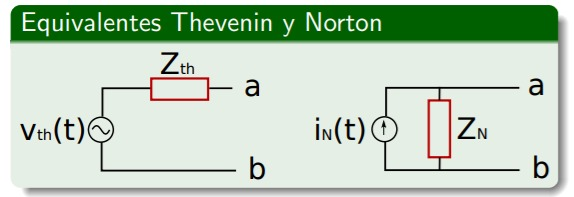
\includegraphics[scale = 0.4]{equivalentes}
	\end{figure}

	\section{Función de transferencia}
	
	\begin{figure}[h]
		\centering
		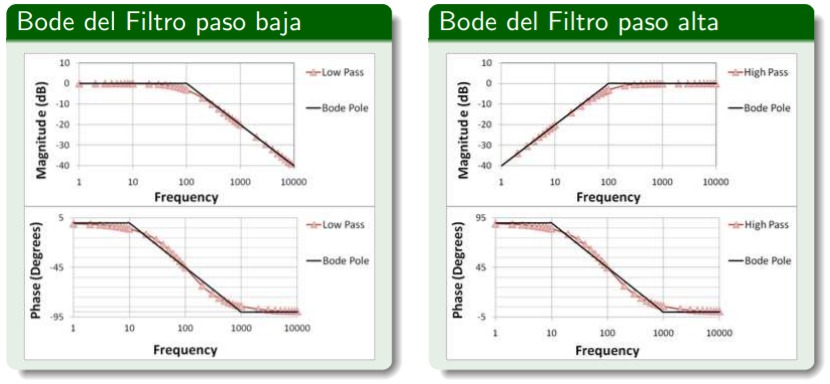
\includegraphics[scale = 0.5]{filtros}
	\end{figure}
	
	
	
\end{document}